\subsection{Visual specification of ontology 2.2}
\begin{figure}[htbp]\centering
\IfFileExists{docs/report/figures/ontology-er-relation-map.png}{%
  \includegraphics[width=\textwidth,height=0.78\textheight,keepaspectratio]{docs/report/figures/ontology-er-relation-map.png}%
}{%
  \includegraphics[width=\textwidth,height=0.78\textheight,keepaspectratio]{figures/ontology-er-relation-map.png}%
}
\caption[Main unique-node ontology map]{Main unique-node ontology map generated from the validated local OWL model. Each local class is rendered exactly once. Solid coloured arrows are asserted domain--range relations; dashed grey links are asserted \texttt{rdfs:subClassOf} axioms. The map uses one representative direction for inverse pairs so that it remains readable; the exact property inventory is documented separately. Coloured regions are presentation modules only and do not add OWL axioms.}\label{fig:ontology-er-relation-map}
\end{figure}

The map is the primary human-readable description of the ontology. It is intentionally closer to an ER/UML or GraphRAG schema than to a raw triple dump: organizations, people, education, governance, ownership and geography are shown as distinct conceptual modules, while every class remains a single node. Its layout is generated deterministically from the Turtle source, not drawn by hand or inferred from a screenshot. The source model is checked independently with the OWL API bundled with Protégé, OWL~2~RL materialization, SHACL validation and SPARQL regression queries. Therefore the figure is a readable projection of checked axioms, not a substitute for the formal validation artifacts.

\begin{figure}[htbp]\centering
\IfFileExists{docs/report/figures/ontology-protege-screenshot.png}{%
  \includegraphics[width=\textwidth]{docs/report/figures/ontology-protege-screenshot.png}%
}{%
  \includegraphics[width=\textwidth]{figures/ontology-protege-screenshot.png}%
}
\caption[Protégé OntoGraf view of ontology 2.2]{Direct screenshot of Protégé 5.6.7 with the OntoGraf plug-in,
after loading the committed \texttt{ontology/vnedu.ttl}. The class hierarchy is shown at left and the
selected ontology graph at right; the graph was laid out by OntoGraf and includes the selected
OWL classes and their asserted subclass relations.}
\label{fig:ontology-overview}
\end{figure}

\begin{figure}[htbp]\centering
\IfFileExists{docs/report/figures/ontology-protege-relations.png}{%
  \includegraphics[width=\textwidth]{docs/report/figures/ontology-protege-relations.png}%
}{%
  \includegraphics[width=\textwidth]{figures/ontology-protege-relations.png}%
}
\caption[Protégé object-property signature]{Direct screenshot of Protégé's Object properties view for
the committed ontology. The selected \term{governedBy} relation is displayed with bilingual labels,
its comment, domain \term{EducationalOrganization}, range \term{GoverningBody}, and its inverse
relation. This is the property-signature view used to verify that the graph has database-like
domain--relationship--range discipline; it is not a hand-drawn diagram.}\label{fig:ontology-protege-relations}
\end{figure}

Protégé is retained as the direct ontology-inspection tool for class and property axioms. GraphDB and Apache Jena Fuseki are retained as execution checks for repository loading, reasoning and SPARQL end-to-end behaviour; their screenshots are intentionally omitted from this section so that the main ontology explanation is not dominated by tool-specific layouts. This separation is important: a workbench layout is a user-interface projection, whereas the OWL axioms, reasoner output and query tests are the evidence for correctness.

\clearpage
\begin{figure}[htbp]\centering
\IfFileExists{docs/report/figures/ontology-tbox-hierarchy-clean.png}{%
  \includegraphics[width=\textwidth,height=0.84\textheight,keepaspectratio]{docs/report/figures/ontology-tbox-hierarchy-clean.png}%
}{%
  \includegraphics[width=\textwidth,height=0.84\textheight,keepaspectratio]{figures/ontology-tbox-hierarchy-clean.png}%
}
\caption[Complete local TBox class hierarchy]{Complete local OWL class hierarchy generated directly from \texttt{ontology/vnedu.ttl}. Every displayed blue arrow is an asserted \texttt{rdfs:subClassOf} triple; disconnected nodes are intentionally retained because the ontology does not assert a superclass for them. Orthogonal routing is used to avoid crossing edges.}\label{fig:tbox-hierarchy-clean}
\end{figure}

The hierarchy and the relation map answer different questions. A root class is not an OWL error under the open-world assumption: it is a class for which this ontology has not asserted a local superclass. In particular, \texttt{Person}, \texttt{AdministrativeUnit}, \texttt{AcademicProgram}, \texttt{FieldOfStudy}, \texttt{OwnershipType} and \texttt{SourceObservation} are independent modelling concepts. The defined classes \texttt{PublicInstitution}, \texttt{PrivateInstitution}, \texttt{MilitaryInstitution} and \texttt{PoliceInstitution} are classified by \texttt{owl:equivalentClass} restrictions rather than by an asserted \texttt{rdfs:subClassOf} edge; adding a superclass only to make a picture connected would change the semantics. If a future competency-questions review confirms that those categories are intended as direct kinds of educational organization, that axiom can be added with a test case; it is not inferred from the visualization requirement.

\clearpage
\begin{figure}[htbp]\centering
\IfFileExists{docs/report/figures/ontology-tbox-signatures-organization.png}{%
  \includegraphics[width=\textwidth,height=0.88\textheight,keepaspectratio]{docs/report/figures/ontology-tbox-signatures-organization.png}%
}{%
  \includegraphics[width=\textwidth,height=0.88\textheight,keepaspectratio]{figures/ontology-tbox-signatures-organization.png}%
}
\caption[Organization and governance signatures]{Exact local object-property signatures for organization, governance, membership, ownership and structural relations. Each row is independent: left box is the declared domain, the diamond is the predicate, and right box is the declared range. No edge is routed through another row.}\label{fig:tbox-signatures-organization}
\end{figure}

\clearpage
\begin{figure}[htbp]\centering
\IfFileExists{docs/report/figures/ontology-tbox-signatures-education.png}{%
  \includegraphics[width=\textwidth,height=0.88\textheight,keepaspectratio]{docs/report/figures/ontology-tbox-signatures-education.png}%
}{%
  \includegraphics[width=\textwidth,height=0.88\textheight,keepaspectratio]{figures/ontology-tbox-signatures-education.png}%
}
\caption[Education and people signatures]{Exact local object-property signatures for programmes, majors, fields, people and educational participation. The missing range of \term{birthPlace} is shown explicitly as unspecified rather than guessed.}\label{fig:tbox-signatures-education}
\end{figure}

\clearpage
\begin{figure}[htbp]\centering
\IfFileExists{docs/report/figures/ontology-tbox-signatures-geography.png}{%
  \includegraphics[width=\textwidth,height=0.70\textheight,keepaspectratio]{docs/report/figures/ontology-tbox-signatures-geography.png}%
}{%
  \includegraphics[width=\textwidth,height=0.70\textheight,keepaspectratio]{figures/ontology-tbox-signatures-geography.png}%
}
\caption[Geography and change signatures]{Exact local signatures for location and province-change relations. The former/current province distinction is represented as a directed relation, not as a timeless equivalence.}\label{fig:tbox-signatures-geography}
\end{figure}

\clearpage
\begin{figure}[htbp]\centering
\IfFileExists{docs/report/figures/ontology-tbox-signatures-other.png}{%
  \includegraphics[width=\textwidth,height=0.38\textheight,keepaspectratio]{docs/report/figures/ontology-tbox-signatures-other.png}%
}{%
  \includegraphics[width=\textwidth,height=0.38\textheight,keepaspectratio]{figures/ontology-tbox-signatures-other.png}%
}
\caption[Other local object-property signature]{The remaining local object property, \term{website}, has an asserted domain but no asserted range in the ontology. This is shown as an open endpoint, not silently assigned \texttt{xsd:anyURI}.}\label{fig:tbox-signatures-other}
\end{figure}

\clearpage
\begin{figure}[htbp]\centering
\IfFileExists{docs/report/figures/abox-instance-neighborhood.png}{%
  \includegraphics[width=\textwidth,height=0.72\textheight,keepaspectratio]{docs/report/figures/abox-instance-neighborhood.png}%
}{%
  \includegraphics[width=\textwidth,height=0.72\textheight,keepaspectratio]{figures/abox-instance-neighborhood.png}%
}
\caption[ABox instance neighborhood for a real university]{Data-driven ABox view generated from the gold serving union. The orange nodes are named individuals: one university, four programmes, four majors, four fields, location units and the reported governing body. Coloured edges are asserted or materialized object-property links; dashed \texttt{rdf:type} edges connect only the most specific visible types to the TBox. This reproducible instance view complements the main unique-node TBox map and the direct Protégé inspection.}\label{fig:abox-instance-neighborhood}
\end{figure}
\clearpage

\subsection{TBox, ABox and constraint semantics}
The ontology is intentionally split into a schema layer and a data layer. The TBox is
\texttt{ontology/vnedu.ttl}: classes, subclass axioms, property signatures, inverse properties,
property chains, defined classes and selected disjointness. The ABox is the generated RDF in
\texttt{data/gold/vnedu-data.ttl}, with \texttt{data/gold/vnedu-all.ttl} as the serving union of
asserted data and materialized entailments. A URI such as
\texttt{university:dai-hoc-bach-khoa-ha-noi} is an individual; \texttt{vnedu:University} and
\texttt{vnedu:HigherEducationInstitution} are classes. Mixing these levels without explicit
\texttt{rdf:type} and \texttt{rdfs:subClassOf} labels is what made the earlier graph misleading.

\begin{longtable}{P{3.4cm}P{6.2cm}P{5.0cm}}
\caption{Separation of ontology axioms, data assertions and validation constraints.}\label{tab:tbox-abox-constraints}\\
\toprule Layer & What is asserted & Correct interpretation \\\midrule\endfirsthead
\toprule Layer & What is asserted & Correct interpretation \\\midrule\endhead
TBox & \texttt{rdfs:subClassOf}, \texttt{rdfs:domain}, \texttt{rdfs:range}, inverses, chains, restrictions and disjointness. & Schema-level meaning and inference rules; it does not require every possible individual to have every field. \\
ABox & Individuals, \texttt{rdf:type}, object-property links, literals, external identifiers and provenance observations. & Source-backed claims; an omitted triple is unknown under the open-world assumption. \\
OWL reasoning & Domain/range and property axioms materialize types and consequences, including inferred superclasses and inverse links. & A wrong domain/range can infer a wrong type; OWL entailment is not a database foreign-key rejection. \\
SHACL & \texttt{shapes/vnedu-shapes.ttl} checks cardinality, datatypes, patterns, temporal intervals and observation structure. & Closed-world data-quality validation, separate from OWL entailments. \\
\bottomrule
\end{longtable}

The design therefore uses domain and range as semantic typing constraints, and SHACL for operational
requirements such as ``at least one provider'' or a valid year range. This is the standards-correct
combination for an RDF/OWL knowledge graph: imposing every relational-database NOT NULL or foreign-key
rule directly in OWL would be unsound under the open-world assumption. Time-dependent legal categories
remain qualified observations rather than permanent global disjointness axioms.

\begin{figure}[htbp]\centering
\begin{tikzpicture}
\node[auditbox] (org) at (0,0) {Organization};
\node[auditbox] (body) at (-5,-1.6) {GoverningBody};
\node[auditbox,text width=4cm] (edu) at (0,-1.6) {EducationalOrganization};
\node[auditbox] (company) at (5,-1.6) {Company};
\node[auditbox,text width=3.5cm] (hei) at (0,-3.4) {HigherEducation\\Institution};
\node[auditbox] (branch) at (5,-3.4) {Branch};
\node[auditbox] (min) at (-5,-3.4) {Ministry / Provincial\\People's Committee};
\node[auditbox,text width=2.7cm] (u) at (-5.25,-5.5) {University};
\node[auditbox,text width=2.7cm] (s) at (-1.75,-5.5) {UniversitySchool};
\node[auditbox,text width=2.7cm] (a) at (1.75,-5.5) {Academy};
\node[auditbox,text width=2.7cm] (o) at (5.25,-5.5) {OfficerSchool};
\foreach \n in {body,edu,company} \draw[auditarr] (\n.north)--(org.south);
\draw[auditarr] (hei)--(edu);
\draw[auditarr] (branch.north)--(edu.south east);
\draw[auditarr] (min)--(body);
\foreach \n in {u,s,a,o} \draw[auditarr] (\n.north)--(hei.south);
\node[font=\small,align=center] at (0,-6.6) {PublicInstitution and PrivateInstitution are defined by ownership values;\\they are orthogonal to the four legal-type classes, not their replacements.};
\end{tikzpicture}

\caption[Organizational class hierarchy]{Selected organizational hierarchy. Arrows point from subclass to superclass.
The four legal-type classes are no longer globally disjoint: an enduring institution can change type.
This is a selected view of \metricClasses{} classes.}\label{fig:taxonomy}
\end{figure}
\begin{figure}[htbp]\centering
\begin{tikzpicture}
\node[auditbox,text width=4cm] (e1) at (0,0) {EducationalOrganization};
\node[auditbox,text width=3.6cm] (g) at (9,0) {GoverningBody};
\draw[auditarr] (e1)--node[auditlabel,above]{governedBy / stateManagedBy}(g);
\node[font=\scriptsize] at (4.5,-0.65) {governedBy inverse: governs; oversight is a separate relation};
\node[auditbox,text width=4cm] (e2) at (0,-1.9) {EducationalOrganization};
\node[auditbox,text width=3.6cm] (p) at (9,-1.9) {Person};
\draw[auditarr] (e2)--node[auditlabel,above]{rector / director / councilChair}(p);
\node[font=\scriptsize] at (4.5,-2.55) {role properties are subproperties of hasLeader; inverse: leads};
\node[auditbox,text width=4cm] (e3) at (0,-3.8) {EducationalOrganization};
\node[auditbox,text width=3.6cm] (prog) at (9,-3.8) {AcademicProgram};
\draw[auditarr] (e3)--node[auditlabel,above]{offersProgram}(prog);
\node[font=\scriptsize] at (4.5,-4.45) {inverse: offeredBy (F)};
\node[auditbox,text width=2.7cm] (pr2) at (0,-5.8) {AcademicProgram};
\node[auditbox,text width=2.6cm] (major) at (4.5,-5.8) {Major};
\node[auditbox,text width=2.7cm] (field) at (9,-5.8) {FieldOfStudy};
\draw[auditarr] (pr2)--node[auditlabel,above]{ofMajor (F)}(major);
\draw[auditarr] (major)--node[auditlabel,above]{inField}(field);
\node[font=\scriptsize,align=center] at (4.5,-6.65) {offersProgram followed by ofMajor entails trainsMajor;\\inField is aligned to skos:broader.};
\end{tikzpicture}

\caption[Property signatures across ontology modules]{Selected domain--property--range signatures.
These arrows are not mandatory foreign keys. Program providers and majors are no longer functional:
multiple values must not force different institutions or subjects to become identical.}\label{fig:relations}
\end{figure}
\begin{figure}[htbp]\centering
\begin{tikzpicture}
\node[auditbox,text width=2.6cm] (u) at (0,0) {Organization $U$};
\node[auditbox,text width=2.6cm] (old) at (4.7,0) {FormerProvince\\$P_o$};
\node[auditbox,text width=2.6cm] (new) at (9.4,0) {Province $P_n$};
\node[auditbox,text width=2.6cm] (region) at (9.4,-2.5) {Region $R$};
\draw[auditarr] (u)--node[auditlabel,above]{locatedIn}(old);
\draw[auditarr] (old)--node[auditlabel,above]{mergedInto}(new);
\draw[auditarr] (new)--node[auditlabel,right]{partOf}(region);
\draw[auditarr,dashed] (u.north) to[out=55,in=125] node[auditlabel,above]{inferred locatedIn} (new.north);
\draw[auditarr,dashed] (u.south)|-node[auditlabel,pos=0.7,above]{inferred locatedIn}(region.west);
\node[font=\small,align=center] at (4.7,-3.6) {A current-boundary crosswalk is not a dated history.\\The analogous bornIn chain does not prove that $P_n$ existed at birth.};
\end{tikzpicture}

\caption[Geographic property-chain inference]{Institution-location inference under the selected administrative
crosswalk. It does not establish historical validity. Birth-area mapping now uses a separate
\term{birthAreaInCurrentCrosswalk} predicate instead of adding historical \term{bornIn} statements.}\label{fig:geo-chain}
\end{figure}

\subsection{Implemented corrections and evidence limits}
The design is standards-based and suitable for an educational knowledge-graph prototype,
but consistency is not a certificate of factual accuracy. Version 2.2 makes the following
changes without reminting existing entity identifiers.
{\small
\begin{longtable}{P{3.7cm}P{6.1cm}P{4.8cm}}
\caption{Ontology 2.2 corrections and their limits.}\label{tab:design-review}\\
\toprule Concern & Implemented correction & Evidence boundary \\\midrule\endfirsthead
\toprule Concern & Implemented correction & Evidence boundary \\\midrule\endhead
Supervision versus inclusion &
Removed parent-organization alignments from governance, subordination, ownership and membership. The branch alignment remains because a branch is a structural subdivision. &
Supervision or investment does not automatically establish organizational parenthood. \\
Direct versus indirect governance &
Added \term{directlyGovernedBy} and \term{reportedGovernedBy} under the broad \term{governedBy}; only the broad relation propagates through superiors. &
Legacy source relations migrate to reported, not unsupported direct, governance. \\
Leadership versus employment &
Removed leader-to-employee and leader-to-\term{worksFor} alignments; added role observations. &
A council chair need not be an employee. \\
Institutional type changes &
Removed global disjointness between the four legal-type classes; added classification observations. &
The class projection is not a dated authoritative legal register. \\
Education versus alumni &
Recorded education becomes \term{educatedAt}, with the neutral inferred class \term{EducationParticipant}. &
Attendance does not entail graduation. Alumni terms remain for explicit evidence. \\
Joint programs &
Removed functionality from \term{offeredBy} and \term{ofMajor}; SHACL requires at least one provider and major. &
Curated program identifiers still do not distinguish all curriculum variants. \\
Birth geography &
Successor and containment chains produce \term{birthAreaInCurrentCrosswalk}, not additional \term{bornIn} facts. &
A current province is not asserted to have existed at birth. \\
Version publication &
Archived 2.1 and 2.2 Turtle; generated HTML, Turtle and JSON-LD version documents and dynamic routes. &
The source and Pages workflow provide the route; stable public uptime still depends on deployment. \\
\bottomrule
\end{longtable}}

\subsection{Standards and conformance assessment}
The audited ontology follows the RDF 1.1/Turtle and OWL 2 RDF serialisation conventions and
uses explicit OWL classes, object properties, datatype properties, inverse properties,
selected functional properties, disjointness, property chains and defined classes. The
current source contains \metricClasses{} local classes, \metricObjectProperties{} local object
properties, \metricDataProperties{} local datatype properties and \metricOntologyTriples{} ontology triples.
The visualisation above is generated from those current source counts, so it can be regenerated
after an ontology change rather than becoming a stale hand-drawn figure.

The design is suitable for a standards-based academic prototype, but it is not an automatic
``five-star'' certification. The following claims are deliberately separated:
\begin{longtable}{P{4.0cm}P{5.6cm}P{5.0cm}}
\caption{Standards assessment and remaining boundaries.}\label{tab:standards-assessment}\\
\toprule Area & Evidence in this release & Honest qualification \\\midrule\endfirsthead
\toprule Area & Evidence in this release & Honest qualification \\\midrule\endhead
RDF and URI design & Stable HTTPS namespace, version IRI, Turtle/JSON-LD/N-Triples publication, content negotiation checks and licence metadata. & Deployment and long-term availability at the canonical origin remain operational responsibilities. \\
OWL 2 modelling & The ontology parses as RDF and passes the OWL API \texttt{OWL2RLProfile} gate with zero violations; inverse relations, chains, restrictions, equivalent classes and selected disjointness remain explicit. & This certifies profile membership of the local ontology, not complete imported-vocabulary semantics or factual correctness. \\
Constraint validation & SHACL shapes validate required fields, datatypes, temporal intervals and observation structure; the current suite reports zero violations under its policy. & Warnings reflect incomplete source coverage; SHACL validation is not proof of factual truth. \\
Provenance and time & PROV-O-style source links and reified evidence observations preserve snapshot context and optional temporal qualifiers. & The current Silver snapshot still lacks claim-level dates for many facts; an undated observation is not a current fact. \\
Vocabulary reuse & Conservative links to Schema.org, FOAF, DBpedia, SKOS, PROV-O and external identifiers. & External ontologies are not fully imported and reasoned over; alignments must remain semantically narrow. \\
Linked Data stars & Machine-readable publication, stable links, external links, licence and open formats are implemented. & The five-star scheme is a publication maturity heuristic, not a formal conformance test, and does not certify accuracy, security or production performance. \\
\bottomrule
\end{longtable}

\subsection{Qualified observations and temporal interpretation}
The transformer creates \metricObservations{} \term{SourceObservation} records, including
leadership, measurement and classification specializations. Each reifies a triple through
\term{rdf:subject}, \term{rdf:predicate} and \term{rdf:object}. Its SHA-256-derived URI includes
the assertion, snapshot digest, source context and qualifiers. Identical evidence preserves
the observation URI; changed evidence creates a different record. Entity URIs remain stable.

\begin{figure}[htbp]\centering
\begin{tikzpicture}
\node[auditbox,text width=4.2cm] (o) at (0,0) {SourceObservation\\Leadership / Measurement / Classification};
\node[auditbox,text width=3.1cm] (s) at (-4.8,-2.1) {Entity\\institution or person};
\node[auditbox,text width=3.1cm] (p) at (0,-2.1) {Predicate\\role, count or type};
\node[auditbox,text width=3.1cm] (v) at (4.8,-2.1) {Value\\person, literal or class};
\draw[auditarr] (o)--node[auditlabel,above left]{rdf:subject}(s);
\draw[auditarr] (o)--node[auditlabel,right]{rdf:predicate}(p);
\draw[auditarr] (o)--node[auditlabel,above right]{rdf:object}(v);
\node[auditbox,text width=4cm] (e) at (-3,-4.4) {Snapshot digest\\entity-level source context};
\node[auditbox,text width=4cm,dashed] (t) at (3,-4.4) {validFrom / validThrough\\referenceYear / unit};
\draw[auditarr] (o.west) to[out=180,in=120] (e.north west);
\draw[auditarr,dashed] (o.east) to[out=0,in=60] (t.north east);
\node[font=\small,align=center] at (0,-5.6) {No supplied dates $\Rightarrow$ unknown validity, not current validity.};
\end{tikzpicture}

\caption[Evidence-qualified temporal observations]{Observation model. Dashed fields are optional and must come
from evidence. Missing dates mean unknown temporal validity. The diagram is schematic;
no dates are fabricated for real officeholders.}\label{fig:observations}
\end{figure}

The implementation supports \term{validFrom}, \term{validThrough}, \term{referenceYear}
and measurement units, validates calendar dates and interval order, and retains normalized
SHA-256 digests of Silver inputs in \term{data/reports/observation-provenance.json}.
Copied source references provide \emph{entity-level context}, not proof that every assertion
occurs in every referenced source. The snapshot digest is not an upstream publication date.

The present Silver snapshot does not retain sufficient temporal qualifiers for these
measurements and appointments. Generated observations explicitly have unknown temporal
validity. The system does not infer today's leadership or a current enrollment total;
the institution infobox displays this limitation. Flat triples remain a source-snapshot
projection. Historical queries must require relevant date bounds on observations;
absence of an end date does not prove an appointment continues.

SHACL checks observation structure, allowed status, digest syntax, date datatypes and
interval ordering. Regression tests also verify that reification alone does not assert
the reified triple. This is a conservative migration, not a complete longitudinal
collection system. Acquiring actual dates, claim-level provenance, foundation events
and authoritative historical classifications remains future work.

\subsection{Competency questions and prohibited conclusions}
\begin{enumerate}
\item A direct body followed by its superior entails broad governance, not a second direct edge.
\item A council chair does not entail employment; an owner does not entail parenthood.
\item Joint providers or majors do not become identical through a program.
\item Recorded education does not entail the alumni class.
\item A current geographic crosswalk does not create a historical birthplace assertion.
\item An undated observation does not answer a date-valid question merely because it is in the latest export.
\end{enumerate}
Rule-engine execution, formal OWL profile membership, domain correctness and empirical
coverage remain distinct claims. The formal OWL 2 RL gate is now asserted only for the
committed release ontology, with its reproducible command and zero-violation evidence
recorded in \term{data/reports/owl2rl-profile.txt}.
